\chapter{Approaching Word2Vec-$\theta$RARes Language Model} \label{approach}

So far we have seen the basisc of Word2Vec model and Echo State Network. We have also seen the functioning and possible limitation of $\theta$RARes model. In this chapter, we extend the $\theta$RARes model and propose the Word2Vec-$\theta$RARes neural language model and also a Word2Vec-ESN classifier to validate the research hypothesis.

\section{Word2Vec-$\theta$RARes Language Model} \label{sec:w2v-esn_model}

This research proposes a Word2Vec-$\theta$RARes language model for TRA task. The proposed model is inspired from the $\theta$RARes model proposed by Hinaut et al. \cite{xavier:2013:RT} for TRA task. Figure \ref{fig:model_arch} shows the architecture of Word2Vec-$\theta$RARes model. Word2Vec-$\theta$RARes model is the combination of Word2Vec model and Echo State Network (ESN). The Word2Vec model is responsible for generating the distributed embeddings of the words in the input sentences. The generated word embeddings can then used as an input to ESN, which further processes these word embeddings to learn and predict the thematic roles of all semantic words in the input sentences.

\begin{figure}[hbtp]
\centering

\includegraphics[width=0.9\linewidth]{model_arch}
\caption[Architecture of Word2Vec-$\theta$RARes model]{\textbf{Architecture of Word2Vec-$\theta$RARes model:} { \small The model, takes the words of a sentence as an input across time. Word2Vec model generates the distributed vector representation of the input word. The generated word vector is then used by ESN for further processing and learns to predict the thematic roles of the input sentence.}}
\label{fig:model_arch}
\end{figure}

\subsection{Model initialization}

Before using the Word2Vec-$\theta$RARes model for TRA task, the Word2Vec model is trained using skip-gram negative sampling \cite{w2v:mikolov_2013_distributed} approach on a general purpose dataset (e.g. Wikipedia) and the domain specific dataset. During the training of Word2Vec model, the low dimensional distributed embeddings for each word in the corpus vocabulary is learned (see section \ref{get_word_embeddings}).

To initialize the ESN, firstly, a reservoir of size $N_{x}$ composed of leaky integrator neurons and \textit{tanh} activation function is created. The input-to-hidden weights ($W^{in}$) and hidden to hidden weights ($W^{res}$) are then generated sparsely and randomly from a Gaussian distribution with mean 0 and variance 1. These weights once initialized are fixed and remains unchanged during training \cite{esn:scholarpedia:2007, esn:practical_guide}. To generate the weights sparsely, a fixed fan-out of $F_{hh}$ and $F_{ih}$ is chosen for hidden-to-hidden and input-to-hidden connections respectively. In other words, each reservoir neuron is connected to $F_{hh}$ other reservoir neurons and each input neurons are connected to only $F_{ih}$ reservoir neurons. 

\subsection{Training model}

Word2Vec-$\theta$RARes language model treats the TRA task as a prediction problem. The objective of this model is to learn and predict the thematic roles of all semantic words in the input sentence. To evaluate the performance of this model meaning error and sentence error metrics are used (see section \ref{sec:evaluation_metrics_1}). The same evaluation metrics was used to evaluate $\theta$RARes model \cite{xavier:2013:RT}. Thus it enable us to compare the performance of both Word2Vec-$\theta$RARes and $\theta$RARes model.



Figure \ref{fig:model_variant_1}), shows the neural comprehension of Word2Vec-$\theta$RARes model for thematic role assignment. Like $\theta$RARes model, a set of closed class words is created prior to training of model. During the training, the sentences are presented to the model one at a time, word-by-word across time. Before presenting a sentence to the model, all the semantic words (not in closed class set) in the sentence are identified and placed in FIFO memory stack (see fig. \ref{fig:model_variant_1}). This memory stack will be used later to decode the output coded meaning of the semantic words to the meaning of input sentence. The readout layer of the model is also teacher-forced with the coded meaning of the input sentence. The size of readout layer thus depends on the maximum number of semantic words a sentence can have in the corpus. A semantic word in a sentence can have one of the four possible roles: Predicate (P), Agent (A), Object (O), Recipient (R). For example, if the sentences in the corpus have a maximum of $N_{sw}$ semantic words then the readout layer size would be $N_{sw} \times 4 $ neurons; where each output neuron encodes the thematic role of a semantic word. The model could also take the topologically modified but equivalent coded meaning of the sentences (see fig\ref{fig:w2v_esn_nv}), where the role of each noun in a sentence is represented with respect to a verb \cite{xavier:2013:RT}. With the topologically modified coded meaning, the readout units contains $N_{noun} \times N_{verb}$, where $N_{noun}$ and $N_{verb}$ are respectively the maximum number of nouns and verbs any sentence could have in the corpus. The output neurons have an activation of 1 if the corresponding thematic roles are present for the sentence, -1 otherwise. 

The Word2Vec model receives the words from an input sentence over time and generates a word vector of $E_{v}$ dimensions which is then used as an input for the ESN. The input layer of ESN uses this word vector as input features for learning and predicting the thematic roles of the semantic words in the sentences. Thus the size of the input layer is same as the dimensionality of word vector i.e. $E_{v}$. The output ofthe reservoir is accumulated for each time step during the presentation of a sentence. The accumulated reservoir states are then linearly combined with readout activations (coded meaning of the input sentence) to learn the reservoir-to-readout ($W^{out}$) weights using linear or ridge regression. The reservoir states of ESN are reset before the presentation of the consequent sentence. Word2Vec-$\theta$RARes model can be operated in two learning modes so that it learns to extract the coded meaning of the semantic words in the sentences.

\begin{enumerate}
\setlength{\itemsep}{\smallskipamount}

\item \textbf{Sentence Continuous Learning (SCL)}: In this learning mode, learning takes place from the beginning of the sentence. In other words, the coded meaning of the input sentence is made available to model from the onset of the first word of the sentence. Thus, the regression is applied with the teacher roles from the onset of the first word in the sentence \cite{xavier:2013:RT}. \label{eg:SCL}

\item \textbf{Sentence Final Learning (SFL)}: In this mode, the learning takes places only at the end of the sentence \cite{xavier:2013:RT}. Hence, the teacher labels are only provided to the network at the end of sentence i.e. from the last word of the sentence. \label{eg:SFL}

\end{enumerate} 

\begin{figure}[hbtp]
\centering
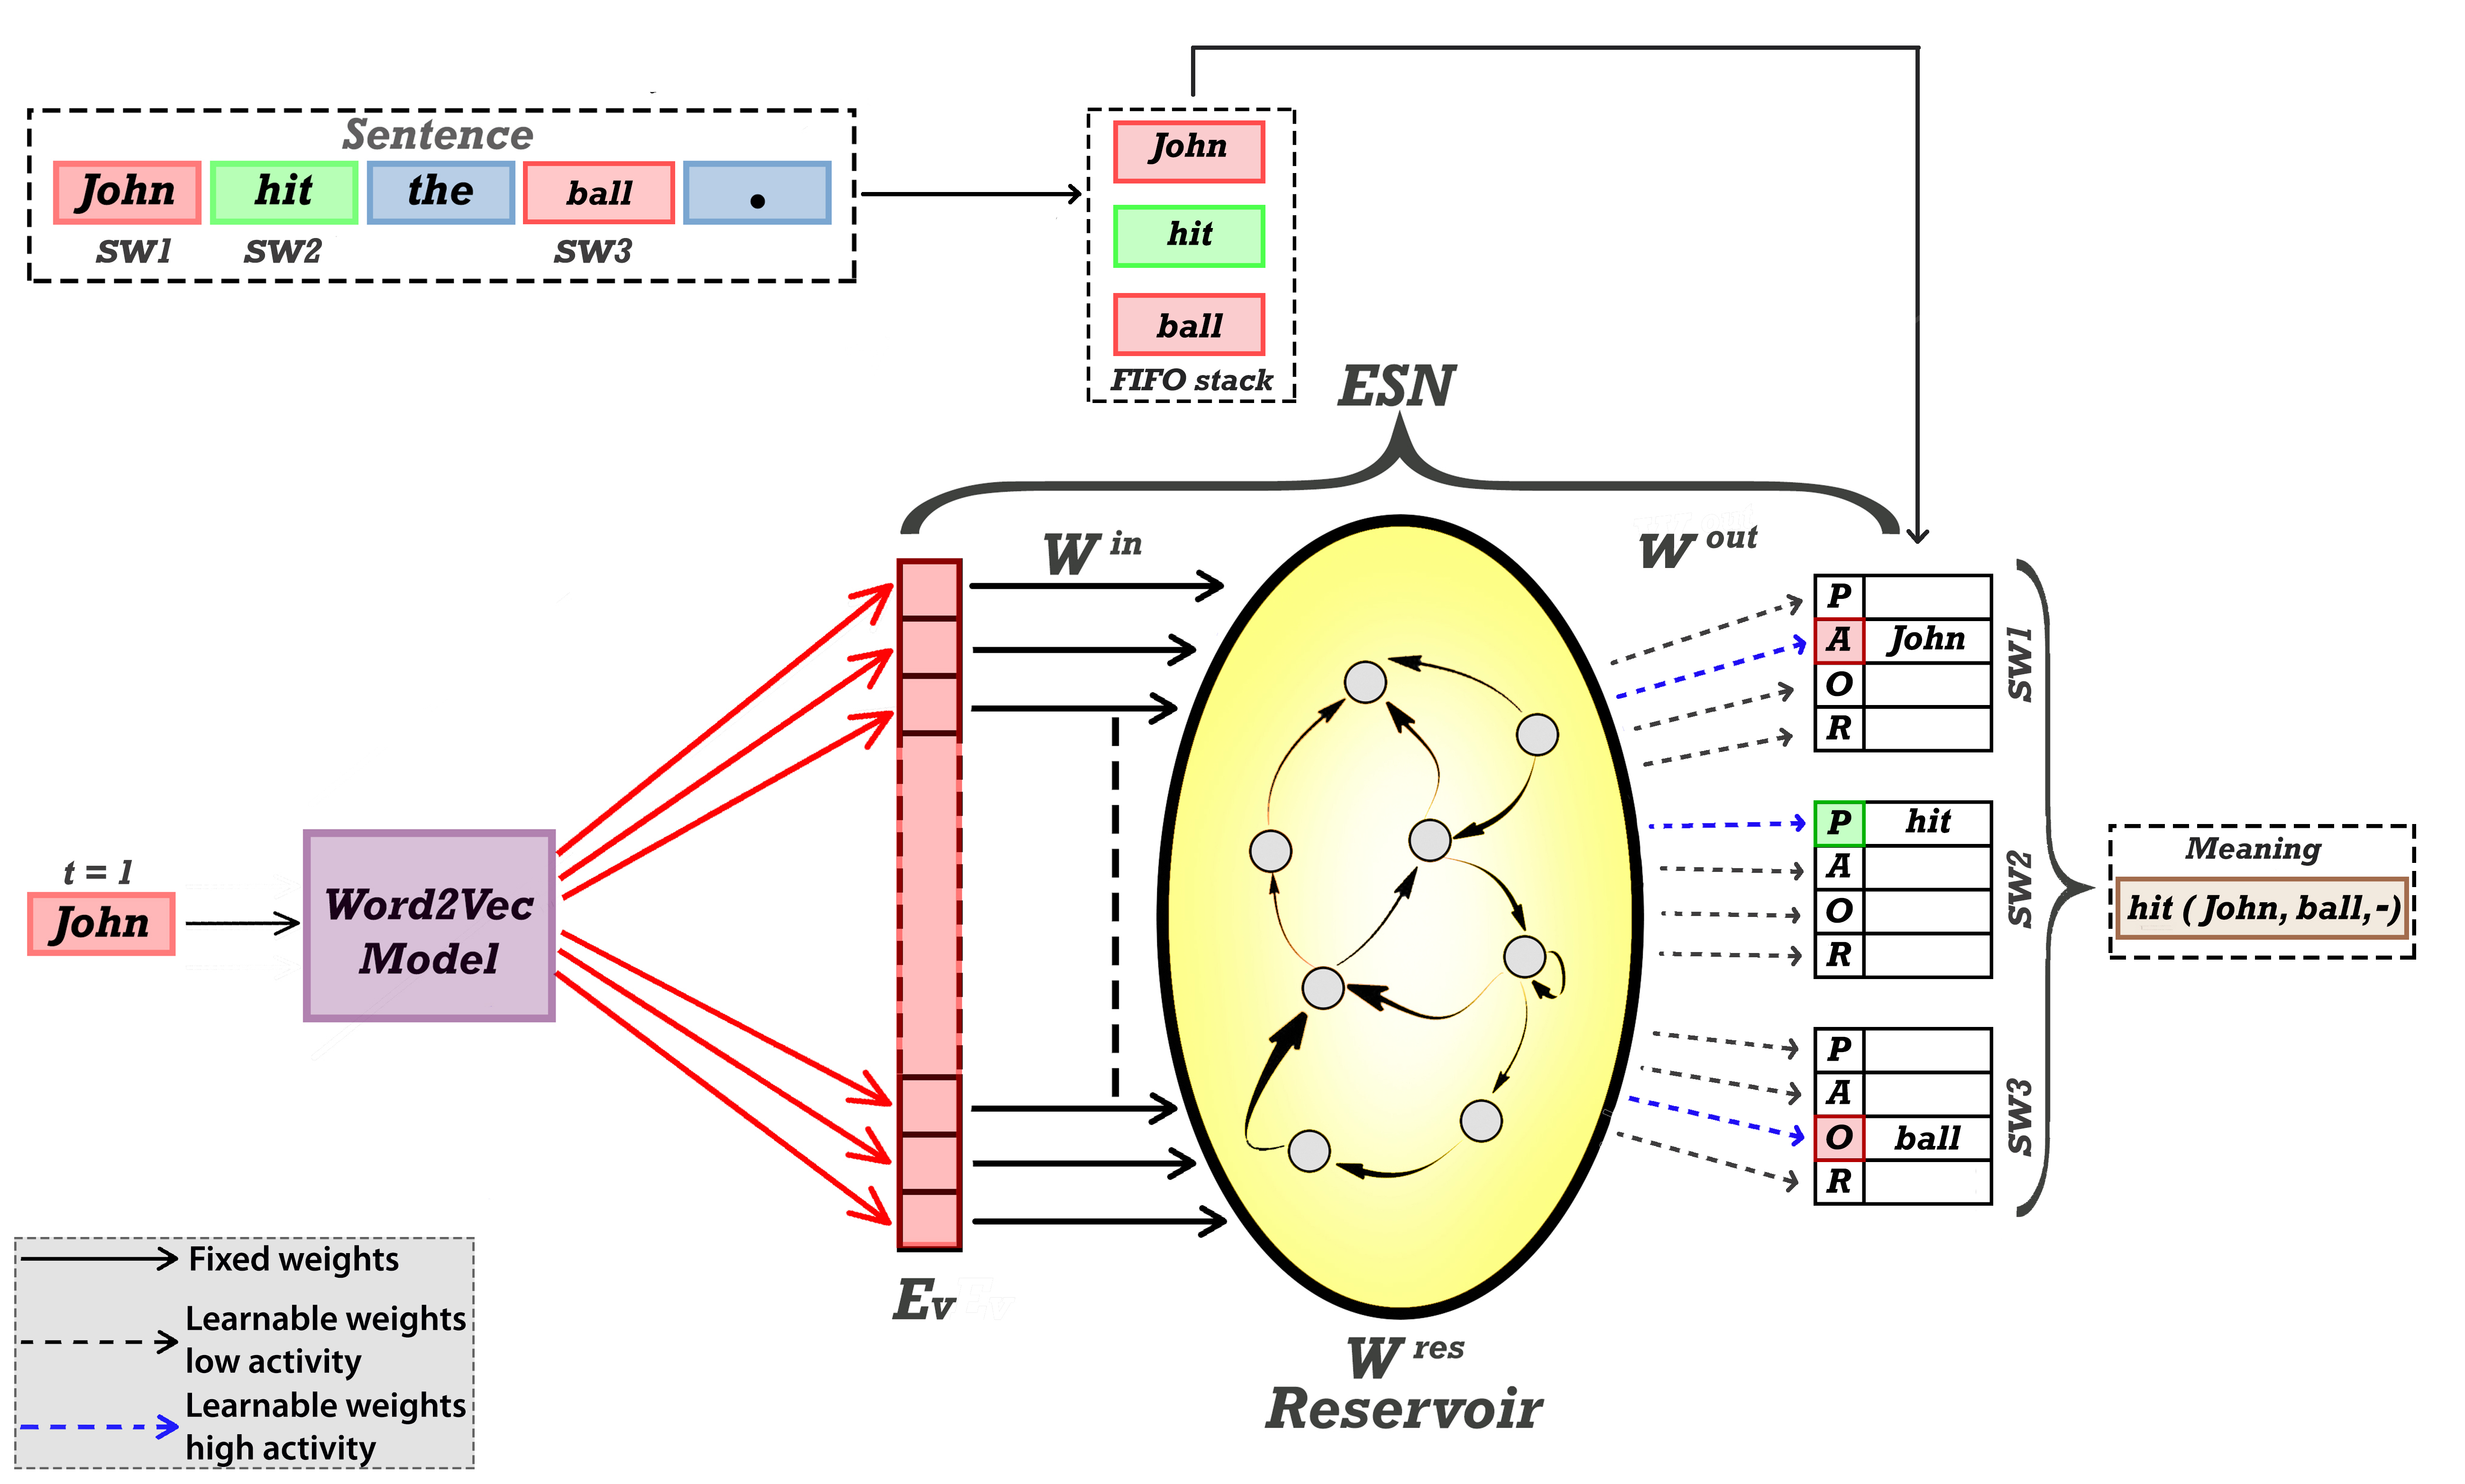
\includegraphics[width=0.9\linewidth]{w2v_esn_model}
\caption[Neural comprehension of Word2Vec-$\theta$RARes Model]{\textbf{Word2Vec-$\theta$RARes language model:} {\small The figure shows the processing of a sentence by the model Word2Vec-ESN classifier at time step 1. Nouns and verbs (specified in red and green respectively) are stored in a memory stack for interpreting the coded meaning. The word \textit{'John'} is input to word2vec model which generate a word vector of $E_{v}$ dimensions. The output vector is then input to ESN for further processing. During training, the readout units are teacher-forced with the coded meaning of the input sentence. During testing, the readout units generate the activations which code the predicted coded meaning of input sentence. The meaning: hit(John, ball, -) is decoded from coded meaning by mapping the thematic roles with semantic words from memory stack. Adapted from \cite{xavier:2013:RT}}} 
\label{fig:model_variant_1}
\end{figure}

\begin{figure}[hbtp]
\centering
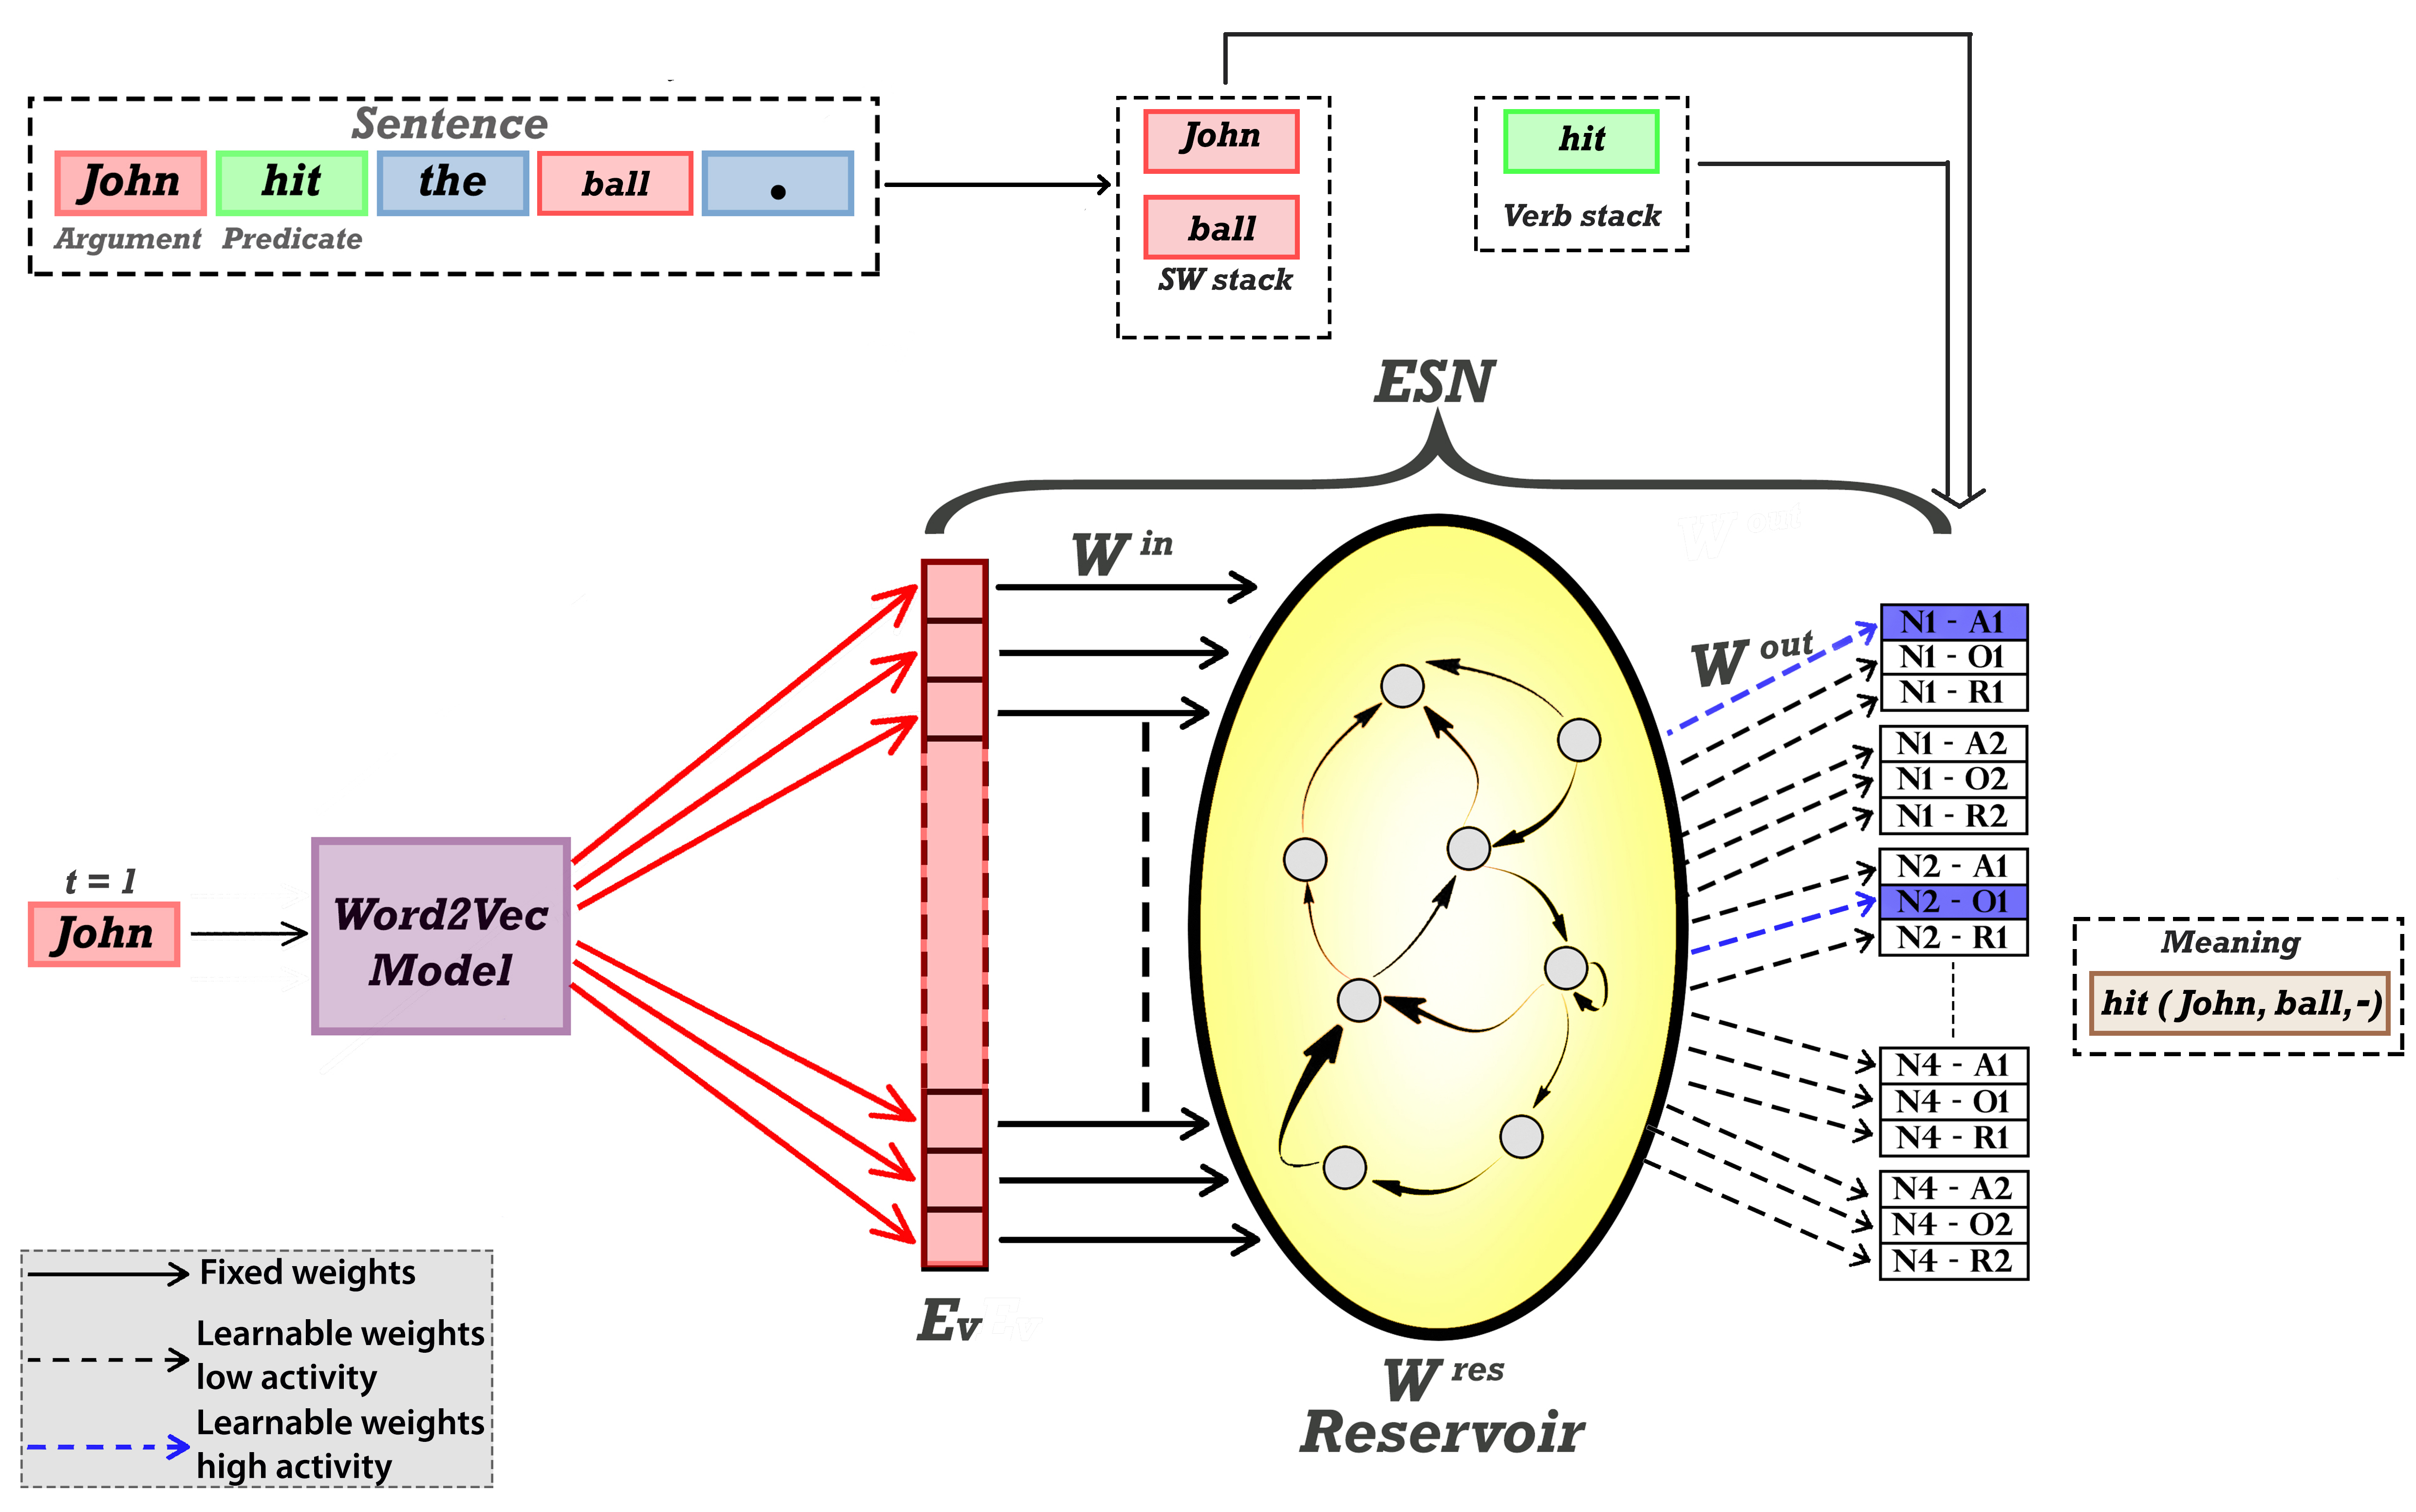
\includegraphics[width=0.9\linewidth]{w2v_esn_nv}
\caption[Neural comprehension of Word2Vec-$\theta$RARes Model]{\textbf{Word2Vec-$\theta$RARes language model with toplogically modified output coding:}{\small The figure shows the processing of a sentence by the model Word2Vec-ESN classifier at time step 1. Nouns and verbs (specified in red and green respectively) are stored in a repective memory stack for interpreting the coded meaning later. The word \textit{'John'} is input to word2vec model which generate a word vector of $E_{v}$ dimensions. The output word vector is then input to ESN for further processing. During training, the readout units are teacher-forced with the coded meaning of the input sentence. The coded meaning ``N1-A1" represents that Noun-1 (`John') is agent of Verb-1 (`hit'). During testing, the readout units generate the activations which code the predicted coded meaning of input sentence. The meaning: hit(John, ball, -) is decoded from coded meaning by mapping the thematic roles with nouns and verbs from memory stack. Adapted from \cite{xavier:2013:RT}} }
\label{fig:w2v_esn_nv}
\end{figure}

\paragraph{Decoding Output: } As described earlier, the coded meaning of a sentence is defined as the description of thematic roles for all the semantic words in the sentence. As the readout neurons of model codes the thematic roles for all semantic words, the output activations produced by the model while testing a sentence are thresholded at 0 for every semantic words. The maximum of all activation between four possible roles (i.e. Predicate, Agent, Object, Recipient) is taken as the coded meaning of a semantic word \cite{xavier:2013:RT}. A semantic word is said to have an incorrect coded meaning if the winning readout neuron is not the true role of the semantic word. If there is no activation above the threshold for a semantic word, then this semantic word is considered to have no coded meaning \cite{xavier:2013:RT}. Combining the coded meaning of semantic words, forms the coded meaning of the sentence. The coded meaning of the sentence can then be decoded to the actual meaning by mapping the coded meaning to the semantic words from the FIFO memory stack(see fig \ref{fig:model_variant_1}).
 
\subsection{Evaluation Metrics}\label{sec:evaluation_metrics_1}

To evaluate the performance of the Word2Vec-$\theta$RARes language model, the same metrics that was used by Hianut et al. \cite{xavier:2013:RT} to evaluate the $\theta$RARes model was employed. The metrics compute the Meaning Error (ME) and the Sentence Error (SE). Meaning error is the percentage of semantic words with incorrect coded meaning, whereas the sentence error is the percentage of sentences having at least one semantic word with incorrect coded meaning. Both the error measures are related, but there is no strict correlation between them \cite{xavier:2013:RT}. Sentence error is a stricter measure than meaning error to evaluate model performance because a meaning error of $5\%$ cannot be used to estimate the sentence error, as this $5 \%$ incorrect words, can be from just one sentence or several sentences. 

To evaluate the performance of Word2Vec-$\theta$RARes model, not all the readout neurons are considered i.e. if a sentence has only three semantic words then only readout neurons corresponding to these three semantic words are analyzed \cite{xavier:2013:RT} and remaining coded meaning of remaining neurons are ignored. It is important to know that if there are more than one verb, in a sentence then each semantic word can have a possible role with respect to each verb. 

\section{Word2Vec-ESN classifier}\label{sec:model_variant}

To ensure the objectivity of our findings apart from Word2Vec-ESN model, this research work also propose a Word2Vec-ESN classifier. Figure \ref{fig:model_variant_2} illustrates the functional organisation of Word2Vec-ESN classifier for TRA task. Although the model Word2Vec-ESN classifier is architecturally (see fig. \ref{fig:model_arch}) similar to Word2Vec-$\theta$RARes model, but varies in training objective and the way the sentences are processed. It treats the TRA task as a classification problem. The training objective of Word2Vec-ESN classifier is to classify the words of the input sentences to one of the roles namely Predicate (P), Agent (A), Object (O), Recipient (R) and No-role (XX) with respect to the verbs and maximize the classification scores for each role (i.e. F1-score, Precision, and Recall- see section-\ref{sec:evaluation_metrics_2}).

Two input features play a major role in Word2Vec-ESN classifier: argument and predicate. An argument describe the current word being processed and the predicate describes the verb with respect to which an argument is processed \cite{end-to-end}. So, if there are $N_{v}$ verbs in a sentence, then the same sentence is processed $N_{v}$ times. Each argument then takes a unique role for an argument-predicate pair. For example in the following sentence there are two predicates namely \textit{`chased'} and \textit{`ate'}. Thus this sentence will be processed twice, and each argument will take a role for an argument-predicate pair \cite{end-to-end}. 

\begin{table}[H]
\centering
\label{tab:argument-predicate}
\begin{tabular}{lccccccccc}
Arguments $\rightarrow$ & the & dog & that & chased & the & cat & ate & the & rat \\
Predicate('chased') 	 & XX  & A   & XX   & P      & XX  & O   & XX  & XX  & XX  \\
Predicate('ate')    	 & XX  & A   & XX   & XX     & XX  & XX  & P   & XX  & O  
\end{tabular}
\end{table}

It is worth noticing that the classifier takes in input, the predicate with respect to which an argument is processed. To retrieve the predicates from a sentence, the Word2Vec-ESN classifier has to depend on syntactic parser e.g. Charniak parser. This limits the classifier from being an end-to-end system for TRA task.  

\begin{figure}[hbtp]
\centering
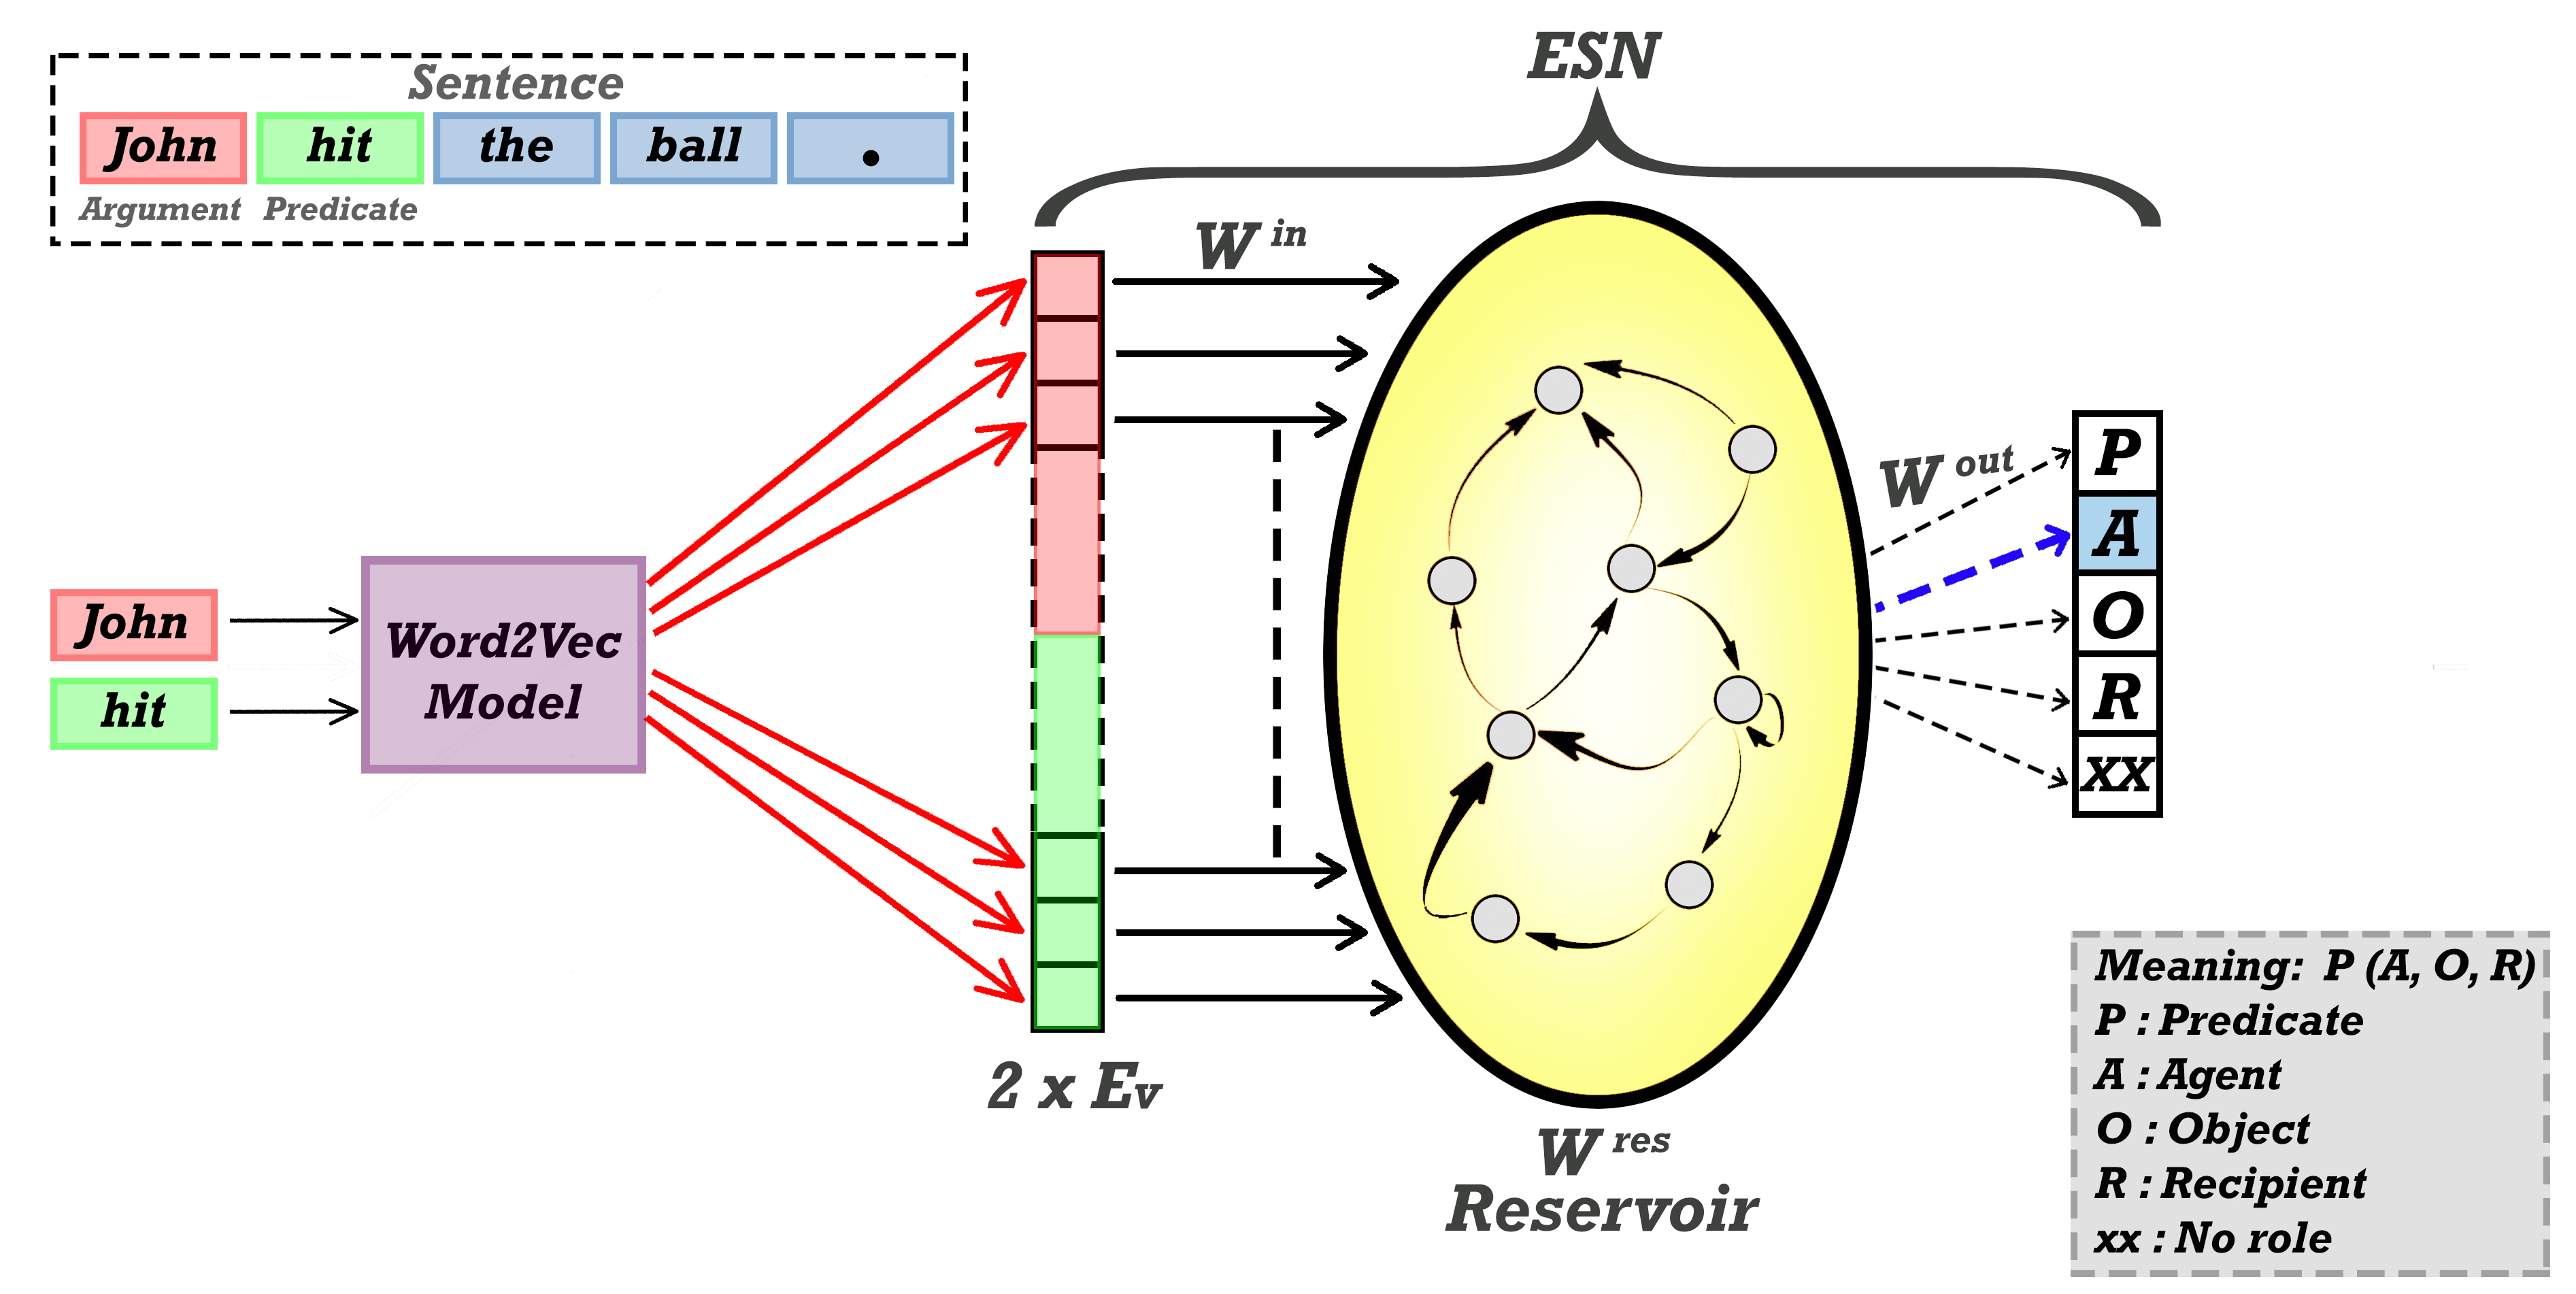
\includegraphics[width=1.0\linewidth]{w2v_esn_variant}
\caption[Functional organisation of Word2Vec-ESN classifier for TRA task] {\textbf{Functional organisation of Word2Vec-ESN classifier for TRA task:} 
{\small The figure shows the processing of a sentence in Word2Vec-ESN classifier at time step 1. At any instant of time, an argument (current word, marked in orange) and predicate (marked in green) is input to the model. Word2Vec model generates the word vectors of $E_{v}$ dimensions which are then concatenated to form a $2 \times E_{v}$ dimensions (shown in red and green color). ESN takes the resultant vector for further processing. During the training, the readout neurons are presented with the role of input word-verb pair (e.g. 'A' for Agent). The read-out weights (shown in dashed line) are learned during training. While testing, the readout unit codes the role of the semantic words, which are then accumulated and decoded to form the meaning \textit{hit(John,ball,--)} of the input sentence at the end. Inspired from \cite{xavier:2013:RT}
}}
\label{fig:model_variant_2}
\end{figure}

\subsection{Training model Word2Vec-ESN classifier}

To train the Word2Vec-ESN classifier, training sentences are presented to the model sequentially. Figure \ref{fig:model_variant_2} shows the processing of an example sentence by Word2Vec-ESN classifier. An input sentence is processed as many time as there are verbs in a sentence, forming multiple sequences. Thus the classifier takes an argument-predicate pair across the time as an input. Unlike Word2Vec-$\theta$RARes model, the readout layer has five neurons each coding for a role (P, A, O, R, XX). Thus during the training, the role of the input argument-predicate pair is also teacher-forced to the model. An output neurons have an activation 1 if an input argument-predicate pair has the corresponding role, -1 otherwise. The Word2vec model initially receives an argument-predicate pair of the input sentence and generates the distributed embeddings for both the input words. The generated word embeddings are concatenated and then taken by ESN as an input. Thus the size of ESN input layer is $2 \times E_{v}$ where the first $E_{v}$ neurons takes the vector representation of the argument and remaining $E_{v}$ neurons for the predicate. The reservoir internal states are collected for an input sequence over time. Reservoir-to-readout ($W^{out}$) weights are then learned by using the linear or ridge regression on collected reservoir states and the readout activations. 

\subsection{Decoding Output}

Recall that the Word2Vec-ESN classifier process a sentence as many times as there are verbs in the sentence. Thus while testing, the output activations of the model is used to predict the role for an argument-predicate pair. The role having the highest output activation is considered as the role of an argument-predicate pair \cite{survey_multi_class}. The role for all argument-predicate pairs is collected and the meaning of the sentence with respect to a verb can then be interpreted by filling up the tagged words in form ``P(A, O, R)". For example, in the sentence ``John hit the ball." as shown in figure \ref{fig:model_variant_2}, the roles for each word-verb pair (i.e. P, A, O, XX ) is used to deduce the meaning of the sentence as ``hit(John, ball, --)".

\subsection{Evaluation Metrics}\label{sec:evaluation_metrics_2}

To analyze the performance of this Word2Vec-ESN classifier on TRA task, the confusion matrix or contingency table \cite{confusion_martrix:1998} is used and the classification scores: Accuracy, Precision, Recall, and F1-Score, are calculated for all possible roles. Higher the classification scores the better. To get the classification score of the model, scores of individual roles are macro-averaged, to get single real numbered scores. The reason for choosing macro-average is that it gives equal weights to all the roles, addressing the role imbalance problem \cite{macro_average:2005}. The same evaluation metrics was also used for CoNLL-04 and CoNLL-05 semantic role labeling shared task \cite{conll:2004,conll:2005}.

\begin{table}[H]
\centering
\caption{Confusion matrix to evaluate Word2Vec-ESN classifier on TRA task.}
\label{tab:argument-predicate}
\begin{tabular}{l|l|c|c|c|c|c|}
\multicolumn{2}{c}{}  &\multicolumn{5}{c}{\textbf{Predicted Roles}}\\
\cline{3-7}
\multicolumn{2}{c|}{} & \textbf{A} & \textbf{O} & \textbf{R} & \textbf{P} & \textbf{XX}\\
\hhline{|~|*6-|}
\multirow{5}{*}{\textbf{True Roles}}
& \textbf{A}     & \cellcolor{gray!25}$TP_{A}$ & $E_{A-O}$ & $E_{A-R}$ & $E_{A-P}$ & $E_{A-XX}$ \\
\hhline{~|*6-}
& \textbf{O}     & $E_{O-A}$ &\cellcolor{gray!25} $TP_{O}$ & $E_{O-R}$ & $E_{O-P}$ & $E_{O-XX}$ \\
\hhline{~|*6-}
& \textbf{R}     & $E_{R-A}$ & $E_{R-0}$ & \cellcolor{gray!25}$TP_{R}$ & $E_{R-P}$ & $E_{R-XX}$ \\
\hhline{~|*6-}
& \textbf{P}     & $E_{P-A}$ & $E_{P-0}$ & $E_{P-R}$ & \cellcolor{gray!25}$TP_{P}$ & $E_{P-XX}$ \\
\hhline{~|*6-}
& \textbf{XX}     & $E_{XX-A}$ & $E_{XX-O}$ & $E_{XX-R}$ & $E_{XX-P}$ & \cellcolor{gray!25}$TP_{XX}$ \\
\hhline{~|*6-}
\end{tabular}
\end{table}

The confusion matrix describes the predictions made by the model. The rows of the matrix correspond to the actual roles and the columns correspond the predictions made by the model. The top left to bottom right diagonal elements of this matrix represent the number of words for which the predicted role is equal to the actual role. So, higher the value of diagonal elements the better. The non-diagonal elements of the matrix represent the number of words which are incorrectly labeled. 

Using the confusion matrix, accuracy can be calculated as the ratio of the number of correctly labeled words to the total number of words (equation \ref{eqn:accuracy}). This accuracy measure specifies how often the classifier is correct \cite{classification_scores:2009}. 

\begin{equation}\label{eqn:accuracy}
Accuracy = \frac{\text{number of words correctly labelled}}{\text{total number of words}}
\end{equation}
 
However, accuracy measure can be distorting (because of accuracy paradox), when the dataset has words with significant role imbalance as it gives high scores to models which merely predict the most frequent class. Thus accuracy measure cannot be used alone to evaluate the performance of the model \cite{accuracy_paradox_1:2008, accuracy_paradox_2:2014}. So, additional performance measures such as Precision (P), Recall(R), and F1-score (F1) are required to evaluate the model. All these measures take a value between 0 and 1. 

\textit{Precision} is defined as the ratio of True positive (TP) to False Positive(FP) and True Positive (equation \ref{eqn:precision}). It is the measure of the accuracy of a role provided that a specific role has been predicted \cite{classification_scores:2009}.

\begin{equation}\label{eqn:precision}
Precision = \frac{\text{True Positive}}{\text{True Positive + False Positive}}
\end{equation}

From the confusion matrix above, the precision for the role Agent($A$) is be calculated as:
\[Precision(A) = \frac{TP_{A}}{(TP_{A}+E_{O-A}+E_{R-A}+E_{P-A}+E_{XX-A})}\]

\noindent \textit{Recall} is defined as the ratio of True Positive to True Positive and False Negative. It measures how good the model is in labeling the correct roles. It is also called \textit{'Sensitivity'} or \textit{'True Positive Rate'}. \cite{classification_scores:2009}.

\begin{equation}\label{eqn:recall}
Recall = \frac{\text{True Positive}}{\text{True Positive + False Negative}}
\end{equation}

Recall for the role `A', from the above confusion matrix is calculate as:
\[Recall(A) = \frac{TP_{A}}{(TP_{A}+E_{A-O}+E_{A-R}+E_{A-P}+E_{A-XX})}\]

\noindent F1-Score or (F1) is the harmonic mean of precision and recall. In other words, it represents the balance between the precision and recall. The F1-score measure takes the false positive and the false negative into consideration. This score is really useful whenever there is a class imbalance in the dataset \cite{classification_scores:2009} and is calculated as:

\begin{equation}\label{eqn:precision}
F1 = 2\times \frac{\text{Precision} \times{Recall }}{\text{Precision + Recall}}
\end{equation}
